% SPDX-License-Identifier: GPL-3.0-or-later
% Copyright (C) 2026 Matías Saavedra
%
% Notes on T. Tachi, "Origamizing Polyhedral Surfaces", IEEE TVCG 16(2), 2010.
% Build: latexmk -pdf -cd docs/tvcg2010-notes.tex  (see CLAUDE.md, Commands)

\documentclass[11pt]{article}

\usepackage[T1]{fontenc}
\usepackage[utf8]{inputenc}
\usepackage{lmodern}
\usepackage{microtype}
\usepackage[margin=2.5cm]{geometry}
\usepackage{amsmath,amssymb,amsthm,mathtools}
\usepackage{booktabs}
\usepackage{enumitem}
\usepackage{tikz}
\usetikzlibrary{calc}
\usepackage{algorithm}
\usepackage{algpseudocode}
\usepackage[hidelinks]{hyperref}

% Deterministic output: no timestamps or random IDs in the PDF, so rebuilding
% an unchanged source reproduces the committed file byte for byte.
\pdfinfoomitdate=1
\pdftrailerid{}

% Let TeX loosen a line rather than overfill it around long code names.
\setlength{\emergencystretch}{2em}

\hypersetup{
  pdftitle={Notes on Tachi, Origamizing Polyhedral Surfaces (TVCG 2010)},
  pdfauthor={Open Origamizer project},
}

\theoremstyle{definition}
\newtheorem{openq}{Open question}
\newtheorem{impl}{Implementation note}
\newtheorem*{reading}{Our reading}

\renewcommand{\theequation}{N\arabic{equation}}

\newcommand{\ETM}{\mathrm{ETM}}
\newcommand{\VTM}{\mathrm{VTM}}
\newcommand{\tv}{\boldsymbol{\theta}}
\newcommand{\wv}{\mathbf{w}}
\newcommand{\Nv}{N_{\mathrm{vert}}}
\newcommand{\Ne}{N_{\mathrm{edge}}}

\title{Notes on Tachi, \emph{Origamizing Polyhedral Surfaces}\\
  \large IEEE TVCG 16(2):298-311, 2010}
\author{Open Origamizer project}
\date{23 November 2026}

\begin{document}
\maketitle

\begin{abstract}
These notes restate the parts of Tachi's 2010 paper~\cite{tvcg10} that the Open
Origamizer implementation needs: the molecule mesh, its parameterization by
angles and widths, the equality and inequality conditions for a valid crease
pattern, the two-step mapping, and edge splitting. They also record
consistency checks we derived, our reading of passages the paper leaves open,
and the questions that must be settled during milestones M1 to M3.
\end{abstract}

\section{Purpose and conventions}

The notes are written from the published paper only, following the project's
clean-room policy. Text and figures are our own; the paper itself is not
redistributed (IEEE copyright). Section numbers such as ``Sec.~4.1'' refer to
the paper.

\begin{itemize}[nosep]
  \item Tags \textup{(T1)} to \textup{(T19)} carry the paper's own equation
    numbers, so that code can cite ``TVCG10 Eq.~7'' and a reader can compare
    with the source.
  \item Tags \textup{(N1)}, \textup{(N2)}, \dots{} mark relations derived in
    these notes. They are not in the paper and need their own unit tests.
  \item \emph{Our reading} marks an interpretation of a passage the paper does
    not make explicit. \emph{Open questions} collect what must be decided
    before or during implementation; Section~\ref{sec:open} lists them all.
\end{itemize}

\begin{table}[ht]
\centering
\small
\begin{tabular}{@{}ll@{}}
\toprule
Symbol & Meaning \\
\midrule
$S$, $V$ & target polyhedral surface; solid it encloses (or a given region behind it) \\
$P$, $F(P)$ & convex planar paper; its folded state \\
$i$, $j$, $o$ & mesh vertices; $o$ is the virtual neighbor standing for the boundary \\
$\ETM(i,j)$, $\VTM(i)$ & edge-tucking molecule of edge $ij$; vertex-tucking molecule of vertex $i$ \\
$\ell(i,j)$ & length of edge $ij$ on $S$ \\
$\alpha(i,j_n)$ & sector angle of $S$ at $i$ between edges $ij_{n-1}$ and $ij_n$ \\
$\theta(i,j)$, $w(i,j)$ & angle and width of $\ETM(i,j)$ seen from $i$ \\
$\Theta_m$ & exterior angle of $\VTM(i)$ at its $m$-th corner \\
$g_i$ & angle defect (Gauss area) $2\pi - \sum_n \alpha(i,j_n)$ \\
$\varphi(i,j)$, $\beta_0(i,j)$, $\beta_1(i,j)$ & angles of the Delaunay triangle of $\VTM(i)$ on the side shared with $\ETM(i,j)$ \\
$\tau(i,j)$, $\tau'(i,j)$ & tuck angle available from the paper; tuck angle required by the tuck proxy \\
$d'(i)$ & length of the joint axis at $i$ (depth of the tuck proxy) \\
$\Nv$, $\Ne$ & number of $\VTM$s; number of $\ETM$s including boundary molecules \\
\bottomrule
\end{tabular}
\caption{Notation, following the paper where it names a quantity.}
\end{table}

\section{Problem and pipeline (Sec.~2)}

Let $S$ be the target surface and $V \supset S$ the solid it encloses. For a
surface with boundary, $V$ is a given finite region behind $S$. The goal is a
crease pattern on a convex polygon $P$ whose folded state satisfies
\[
  S \subset F(P) \subset V ,
\]
so every part of the paper that is not on $S$ is hidden behind it. A convex $P$
can itself be folded from any square that contains it by folding the excess
behind; the smallest such square defines the efficiency (Sec.~9.2.3,
Section~\ref{sec:results} here). The method has three steps (Sec.~2.2):
\begin{enumerate}[nosep]
  \item cut $S$ along mesh edges into a topological disk, a polygonal schema
    (Sec.~2.2.1 and~8.1);
  \item map every polygon of $S$ congruently into the plane, leaving gaps
    between them (Sec.~2.2.2 and~6);
  \item fill the gaps with tucking molecules whose crease patterns glue the
    separated edges and vertices back together when folded (Sec.~2.2.3 and~3).
\end{enumerate}

\section{The molecule mesh (Sec.~3)}

The plane is tessellated into three kinds of cells, together called the
\emph{molecule mesh}:
\begin{itemize}[nosep]
  \item \emph{surface polygons}, congruent copies of the faces of $S$;
  \item \emph{edge-tucking molecules} $\ETM(i,j)$, one per interior edge $ij$
    of the cut surface, each a quadrilateral between the two copies of $ij$;
  \item \emph{vertex-tucking molecules} $\VTM(i)$, one per vertex $i$: an
    $N$-gon, $N$ the valency of $i$, surrounded by the $N$ molecules
    $\ETM(i,j)$. Its corners are the copies of $i$, which fold to one point.
\end{itemize}
A \emph{digon} is a degenerate surface polygon with two vertices and two edges,
both copies of one mesh edge. It has zero area and is mapped to a segment of
length $\ell(i,j)$. Digons appear in boundary preprocessing (Sec.~5.1) and in
edge splitting (Sec.~7).

\subsection{Edge-tucking molecules (Sec.~3.1)}

Let surface polygons $P_0$ and $P_1$ share edge $AB$ of $S$, with copies
$A_0B_0$ and $A_1B_1$ in the plane. In general the quadrilateral
$A_0B_0B_1A_1$ admits a crease pattern that folds $A_0B_0$ onto $A_1B_1$ if and
only if it is simple with positive signed area and
$\min(|A_0B_1|, |A_1B_0|) \ge |AB|$. TVCG10 restricts itself to
\emph{symmetric} molecules with $A_0A_1 \parallel B_0B_1$: an isosceles
trapezoid whose legs are the two copies of the edge (Figure~\ref{fig:etm}). Its
crease pattern is then a single valley fold by $+\pi$ along the symmetry axis,
which reflects one leg onto the other. The legs become the creases between the
polygons and the tuck (mountain when seen from the clean side); their fold
angles follow from the 3D configuration (Sec.~4.3).

\begin{figure}[ht]
\centering
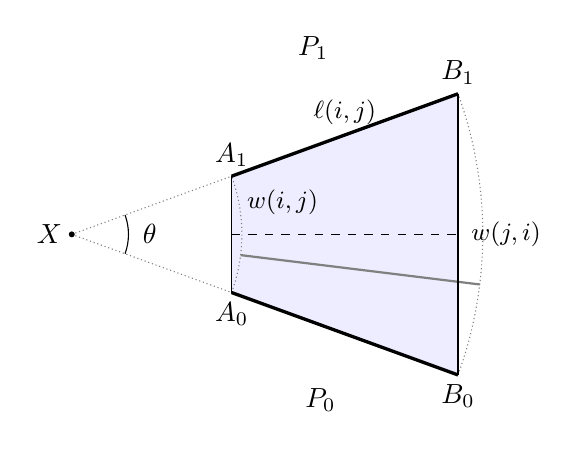
\begin{tikzpicture}[scale=0.9]
  \def\h{20}   % half of theta(i,j), in degrees
  \def\r{2.4}  % distance from the apex X to the corners on the VTM(i) side
  \def\R{5.8}  % \r + ell(i,j)
  \coordinate (X)  at (0,0);
  \coordinate (A0) at (-\h:\r);
  \coordinate (A1) at (\h:\r);
  \coordinate (B0) at (-\h:\R);
  \coordinate (B1) at (\h:\R);
  \fill[blue!7] (A0) -- (B0) -- (B1) -- (A1) -- cycle;
  \draw[densely dotted, gray] (X) -- (A0) (X) -- (A1);
  \draw[densely dotted, gray] (A0) arc[start angle=-\h, end angle=\h, radius=\r];
  \draw[densely dotted, gray] (B0) arc[start angle=-\h, end angle=\h, radius=\R];
  \draw[gray, thick] (-\h+13:\r) -- (-\h+13:\R);
  \draw[very thick] (A0) -- (B0) (A1) -- (B1);
  \draw (A0) -- (A1) (B0) -- (B1);
  \draw[dashed] ($(A0)!0.5!(A1)$) -- ($(B0)!0.5!(B1)$);
  \draw (-\h:0.8) arc[start angle=-\h, end angle=\h, radius=0.8];
  \node at (0:1.1) {$\theta$};
  \fill (X) circle (1.2pt) node[left] {$X$};
  \node[below] at (A0) {$A_0$};
  \node[above] at (A1) {$A_1$};
  \node[below] at (B0) {$B_0$};
  \node[above] at (B1) {$B_1$};
  \node[anchor=west, font=\small] at ($(A0)!0.78!(A1) + (0.08,0)$) {$w(i,j)$};
  \node[anchor=west, font=\small] at ($(B0)!0.5!(B1) + (0.05,0)$) {$w(j,i)$};
  \node[above, sloped, font=\small] at ($(A1)!0.5!(B1)$) {$\ell(i,j)$};
  \node at ($(A1)!0.5!(B1) + (\h+90:1.3)$) {$P_1$};
  \node at ($(A0)!0.5!(B0) + (-\h-90:1.0)$) {$P_0$};
\end{tikzpicture}
\caption{A symmetric edge-tucking molecule $\ETM(i,j)$ (our drawing). The legs
$A_0B_0$ and $A_1B_1$ (thick) are the copies of edge $ij$ in the polygons $P_0$
and $P_1$; extended, they meet at the apex $X$ with angle $\theta(i,j)$. Side
$A_0A_1$ borders $\VTM(i)$, side $B_0B_1$ borders $\VTM(j)$. The dashed axis is
the valley crease. Dotted arcs: where the endpoints of a digon inserted by edge
splitting can lie (gray segment, Section~\ref{sec:split}).}
\label{fig:etm}
\end{figure}

\subsection{Vertex-tucking molecules (Sec.~3.2)}

$\VTM(i)$ must fold all its corners onto one point. Its crease pattern comes
from \emph{Voronoi folding}, which generalizes folding the corners of a triangle
onto its circumcenter along the perpendicular bisectors of the sides:
\begin{enumerate}[nosep]
  \item valley creases ($+\pi$) along the Voronoi diagram of the molecule's
    corners;
  \item mountain creases from each Voronoi vertex to the corners that generate
    its cells, with fold angles given by the tuck proxy (Sec.~4.3);
  \item crimp folds so that the folded tuck follows the curvature of $S$ at $i$
    (Sec.~4.3).
\end{enumerate}
For a convex molecule the Voronoi vertices are the circumcenters of the Delaunay
triangles of its corners. This is why Delaunay angles appear in the conditions
of Section~\ref{sec:2d}.

\section{Parameterization and equality conditions (Sec.~4.1)}

With isometric polygons and symmetric molecules, the molecule mesh is described
by two numbers per edge-tucking molecule (Figure~\ref{fig:etm}):
\begin{itemize}[nosep]
  \item $\theta(i,j)$, the angle between the two copies of edge $ij$, signed by
    the sense of rotation about $i$;
  \item $w(i,j)$, the signed length of the side that $\ETM(i,j)$ shares with
    $\VTM(i)$; a negative value means the molecule is crossed or flipped.
\end{itemize}
For an isosceles trapezoid with legs of length $\ell(i,j)$,
\begin{equation*}
  \theta(j,i) = -\theta(i,j), \qquad
  w(j,i) = w(i,j) + 2\,\ell(i,j) \sin\tfrac12\theta(i,j).
  \tag*{(Sec.~4.1)}
\end{equation*}
For $\theta(i,j) > 0$ the apex lies on the side of $\VTM(i)$; with $r = |XA_0|$,
\begin{equation}
  w(i,j) = 2r \sin\tfrac12\theta(i,j), \qquad
  w(j,i) = 2\bigl(r + \ell(i,j)\bigr) \sin\tfrac12\theta(i,j),
  \label{eq:apex}
\end{equation}
which gives the relation above; $\theta(i,j) < 0$ follows by exchanging $i$ and
$j$. So $\theta(i,j) > 0$ means that the molecule widens from $i$ to $j$. We use
this as the operational sign convention.

Around vertex $i$, let $j_0, \dots, j_{N-1}$ be its neighbors in
counterclockwise order, including $o$ for a boundary vertex, and let
$\alpha(i,j_n)$ be the sector angle of $S$ at $i$ between $ij_{n-1}$ and $ij_n$
(indices modulo $N$). The equality conditions are
\begin{align}
  \sum_{n=0}^{N-1} \theta(i,j_n) &= 2\pi - \sum_{n=0}^{N-1} \alpha(i,j_n),
  \tag{T1}\label{T1}\\
  \sum_{n=0}^{N-1} w(i,j_n)
    \begin{bmatrix} \cos \sum_{m=1}^{n} \Theta_m \\
                    \sin \sum_{m=1}^{n} \Theta_m \end{bmatrix}
  &= \begin{bmatrix} 0 \\ 0 \end{bmatrix},
  \tag{T2}\label{T2}\\
  \Theta_m &= \tfrac12\theta(i,j_{m-1}) + \alpha(i,j_m) + \tfrac12\theta(i,j_m).
  \tag{T3}\label{T3}
\end{align}
$\Theta_m$ is the exterior (turning) angle of $\VTM(i)$ at its corner between
the sides it shares with $\ETM(i,j_{m-1})$ and $\ETM(i,j_m)$. Summing \eqref{T3}
shows that \eqref{T1} says the turning angles of $\VTM(i)$ add up to $2\pi$: the
molecule closes in angle. \eqref{T2} says it closes in position. The right side
of \eqref{T1} is the angle defect $g_i$ of $S$ at $i$; the molecules around $i$
absorb exactly that angle.

\paragraph{Check of \eqref{T3}.} At the corner of $\VTM(i)$ between
$\ETM(i,j_{m-1})$ and $\ETM(i,j_m)$, the full angle $2\pi$ splits into the
polygon corner $\alpha(i,j_m)$, the two trapezoid corners
$\frac{\pi}{2} + \frac12\theta(i,j_{m-1})$ and
$\frac{\pi}{2} + \frac12\theta(i,j_m)$, and the interior angle of $\VTM(i)$.
Hence
\begin{equation}
  \text{interior angle of } \VTM(i) \text{ at corner } m = \pi - \Theta_m ,
  \label{eq:interior}
\end{equation}
with $\Theta_m$ as in \eqref{T3}.

\subsection{Boundary molecules}

For a vertex $i$ on the boundary of the cut surface, TVCG10 attaches a
\emph{boundary molecule} $\ETM(i,o)$ with variables $\theta(i,o)$ and $w(i,o)$
(Sec.~4.1, Fig.~8(b) there), so that every $\VTM$ is surrounded by polygons and
molecules.

\begin{reading}
$o$ sits in the counterclockwise order around $i$ between the two boundary
edges at $i$. $\ETM(i,o)$ has those two boundary-edge copies as legs and stands
for the outside of the paper: its side of length $w(i,o)$ on $\VTM(i)$ lies on
the boundary of $P$. The sector angles next to $o$ are the corner angles of the
first and last polygons at $i$, so $\sum_n \alpha(i,j_n)$ in \eqref{T1} is the
total angle of $S$ at $i$. With legs at angle $\theta(i,o)$, the paper boundary
turns by $\theta(i,o) - \pi$ at boundary vertex $i$ and runs straight along the
boundary-edge copies in between, so \eqref{T4} below is local convexity of $P$.
\end{reading}

\paragraph{Consistency check (Gauss-Bonnet).} Sum \eqref{T1} over all vertices.
Every interior molecule contributes $\theta(i,j) + \theta(j,i) = 0$, so only the
boundary molecules remain:
$\sum_{i \in \partial} \theta(i,o) = \sum_i g_i$. For a polyhedral disk the
discrete Gauss-Bonnet theorem gives
$\sum_{\text{interior}} (2\pi - \sum\alpha) + \sum_{\partial} (\pi - \sum\alpha) = 2\pi$,
hence
\begin{equation}
  \sum_{i \in \partial} \bigl(\theta(i,o) - \pi\bigr) = 2\pi .
  \label{eq:gaussbonnet}
\end{equation}
The turning angles of the paper boundary add up to one full turn, as they must
for a simple closed polygon; this supports the reading above. The same sum
shows why $S$ must be cut: for a closed surface there are no boundary molecules,
so the left side is $0$ while $\sum_i g_i = 2\pi\chi(S)$, which is $4\pi$ for a
sphere.

\section{2D inequality conditions (Sec.~4.2)}\label{sec:2d}

\subsection{Convex paper and no overlap (Sec.~4.2.1)}

For every boundary molecule,
\begin{align}
  \theta(i,o) &\ge \pi, \tag{T4}\label{T4}\\
  w(i,o) &\ge 0. \tag{T5}\label{T5}
\end{align}
Because the boundary of the molecule mesh is then convex, the mesh cannot
overlap unless some cell intersects itself or flips; it is enough that every
molecule is a simple polygon. TVCG10 uses the sufficient conditions
\begin{align}
  -\pi < \theta(i,j) &< \pi, \tag{T6}\label{T6}\\
  \min\bigl(w(i,j), w(j,i)\bigr) &\ge 0 \tag{T7}\label{T7}
\end{align}
for every $\ETM(i,j)$, and
\begin{equation}
  0 \le \Theta_m < \pi \tag{T8}\label{T8}
\end{equation}
for every corner of every $\VTM(i)$. \eqref{T7} and \eqref{T8} make every
vertex-tucking molecule convex (by~\eqref{eq:interior}).

\subsection{Crease pattern validity (Sec.~4.2.2)}

Trapezoidal $\ETM$s always carry a valid pattern, and a convex $\VTM$ has a well
defined Voronoi pattern. What remains is that the patterns of two adjacent
$\VTM$s must not cross inside the $\ETM$ between them. This happens when a
Voronoi vertex of $\VTM(i)$, the circumcenter of a Delaunay triangle, lies too
far beyond the side shared with $\ETM(i,j)$. Let $\varphi(i,j)$ be the angle
opposite that side in the Delaunay triangle of the corners of $\VTM(i)$ that
contains it ($\varphi > \pi/2$ puts the circumcenter beyond the side). The
sufficient condition is
\begin{equation}
  \varphi(i,j) \le \gamma(i,j) + \tfrac{\pi}{2},
  \qquad
  \gamma(i,j) = \gamma(j,i) = \arctan
    \frac{2\,\ell(i,j)\cos\frac12\theta(i,j)}{w(i,j) + w(j,i)} ,
  \tag{T9}\label{T9}
\end{equation}
where $\gamma(i,j)$ is the angle between the side and a diagonal of the
trapezoid. (In the paper the formula for $\gamma$ is a separate, unnumbered
display.) It follows from the trapezoid's height
$\ell(i,j)\cos\frac12\theta(i,j)$ and the horizontal offset
$\frac12\bigl(w(i,j) + w(j,i)\bigr)$ between the endpoints of a diagonal:
\begin{equation}
  \tan\gamma(i,j) =
  \frac{\ell(i,j)\cos\frac12\theta(i,j)}{\frac12\bigl(w(i,j) + w(j,i)\bigr)} .
  \label{eq:gamma}
\end{equation}

\section{3D inequality conditions (Sec.~4.3)}

The folded tuck must not intersect itself, must lie in $V$, and must make the
folded polygons follow the curvature of $S$. Instead of modeling every degree of
freedom of the folded paper, TVCG10 requires the tuck to lie in a precomputed
\emph{tuck proxy} and derives sufficient conditions from it.

\subsection{Tuck proxy (Sec.~4.3.1)}

From every vertex $i$ a ray is shot into $V$: the \emph{joint axis}. It is
trimmed by an inward offset of $S$, so that the proxy does not intersect itself;
its length is $d'(i)$. For every edge $ij$, the joint axes of $i$ and $j$ are
joined by a strip of two triangles. The tuck proxy is the union of these strips.

For comparison, the SoCG 2017 construction~\cite{socg17} calls its proxy a
waffle and places its walls in the dihedral bisector planes (Sec.~3 there).
TVCG10 does not say how the ray direction is chosen
(Open question~\ref{oq:axis}).

\subsection{Tuck angle (Sec.~4.3.2)}

The 2D conditions let $\VTM(i)$ fold so that its corners meet and the adjacent
edges connect. The folded tuck is first crimp-folded so that the ends of the
strips lie along the joint axis; the \emph{tuck angle}, between the joint axis
and the edge, is then adjusted by a further crimp. A crimp can decrease the tuck
angle but not increase it. So the tuck angle $\tau(i,j)$ available from the
folded paper must be at least the angle $\tau'(i,j)$ between the joint axis at
$i$ and edge $ij$ in the tuck proxy. The paper writes this as
\begin{equation}
  \varphi(i,j) - \tfrac12\theta(i,j) \le \pi - \tau'(i,j),
  \tag{T10}\label{T10}
\end{equation}
which means the available tuck angle is
\begin{equation}
  \tau(i,j) = \pi - \varphi(i,j) + \tfrac12\theta(i,j).
  \label{eq:tau}
\end{equation}

\subsection{Tuck width (Sec.~4.3.3)}

The folded molecules must fit in the proxy. For $\ETM(i,j)$, the crease that
folds onto the joint axis has a length $d_{\mathrm{edge}}(i,j) \le d'(i)$, which
the paper rewrites as
\begin{equation}
  w(i,j) \le 2 \sin\bigl(\tau'(i,j) - \tfrac12\alpha(i,j)\bigr)\, d'(i).
  \tag{T11}\label{T11}
\end{equation}
For $\VTM(i)$, its depth $d_{\mathrm{vert}}(i)$, the largest distance from $i$
of a point of the folded molecule projected onto the joint axis, must satisfy
\begin{equation}
  d_{\mathrm{vert}}(i) \le d'(i). \tag{T12}\label{T12}
\end{equation}
\eqref{T12} reduces to \eqref{T11} with an \emph{open sink}: a sink fold, in
which all creases on the reflection plane have the same assignment, about a
plane perpendicular to the joint axis at depth $\max_j d_{\mathrm{edge}}(i,j)$.
It sets $d_{\mathrm{vert}}(i) = \max_j d_{\mathrm{edge}}(i,j)$, keeps the paper
developable, and still lets the $\ETM$s rotate about the joint axis. The paper
does not derive \eqref{T11} (Open question~\ref{oq:t11}).

\section{Preprocessing (Sec.~5)}

\paragraph{Boundary (Sec.~5.1).} To keep \eqref{T4} from overconstraining the
boundary, TVCG10 adds an extra $\ETM$, a $\VTM$, and a digon to each boundary
edge. Our reading of the figure: the digon is glued along the boundary edge
through the new $\ETM$, so the old boundary edge becomes interior and gains a
free angle, and the paper boundary moves to the outer copies of the boundary
edges. The exact bookkeeping is Open question~\ref{oq:boundary}.

\paragraph{Triangulation (Sec.~5.2).} At a concave corner of a polygon at $i$,
between $\ETM(i,j_0)$ and $\ETM(i,j_1)$, the following necessary conditions for
\eqref{T10} fail:
\begin{align}
  \tau'(i,j_0) + \tau'(i,j_1) &< 2\pi - \alpha(i,j_1), \tag{T13}\label{T13}\\
  \max\bigl(\tau'(i,j_0), \tau'(i,j_1)\bigr) &< \pi. \tag{T14}\label{T14}
\end{align}
So concave polygons are triangulated. TVCG10 triangulates convex polygons too,
because the extra molecules make the conditions easier to meet, but the mapping
also works with quadrilaterals (Sec.~9).

\begin{impl}
We split only nonconvex faces by default (CLAUDE.md, M1). Each added diagonal
becomes an $\ETM$, that is, a potential tuck across the face, which conflicts
with one rigid tile per facet in the fabrication track. Full triangulation stays
available as an option when the mapping fails.
\end{impl}

\section{Mapping (Sec.~6)}

\subsection{Variables (Sec.~6.1)}

Number the $\ETM$s, boundary molecules included, as $n = 1, \dots, \Ne$, each
with a fixed orientation $i \to j$. The unknowns are $\tv, \wv \in \mathbb
R^{\Ne}$ with
\[
  \theta_n = \theta(i,j), \qquad w_n = \min\bigl(w(i,j), w(j,i)\bigr),
\]
and $w_n = w(i,o)$ for a boundary molecule. \eqref{T1} and \eqref{T2} are
$3\Nv$ equations in $2\Ne$ unknowns. With all polygons triangulated and the
boundary preprocessed, the paper states $\Nv = \frac13 \Ne + 1$, leaving
$\Ne - 3$ degrees of freedom (Open question~\ref{oq:dof}). The mapping fixes the
rotations of the polygons first ($\tv$) and then their translations ($\wv$),
which makes \eqref{T2} linear.

\subsection{Rotation step (Sec.~6.2)}

\eqref{T1} for all vertices reads
\begin{equation}
  C_\theta \tv = \mathbf g, \tag{T15}\label{T15}
\end{equation}
where $C_\theta$ is $\Nv \times \Ne$ with one row per vertex: $+1$ for
molecules oriented away from the vertex, $-1$ for molecules oriented toward it
(since $\theta(j,i) = -\theta(i,j)$), and $+1$ for its boundary molecule;
$g_i$ is the angle defect. The solutions are
\begin{equation}
  \tv = C_\theta^+ \mathbf g + \bigl(I - C_\theta^+ C_\theta\bigr)\tv_0,
  \qquad C_\theta^+ = C_\theta^\top \bigl(C_\theta C_\theta^\top\bigr)^{-1},
  \tag{T16}\label{T16}
\end{equation}
with $\tv_0$ free, a space of dimension $\Ne - \Nv$. The inequalities
\eqref{T4}, \eqref{T6}, and \eqref{T8} are linear in $\tv$, since $\Theta_m$ is
linear by \eqref{T3}. TVCG10 minimizes $E_\theta$, the sum of squared violations
of these inequalities, by gradient descent with a line search, projecting each
step onto the null space of $C_\theta$. The problem is convex, so the descent
reaches the global minimum; in every model the author tested that minimum was
zero, which the paper notes is observed but not proved.

\subsection{Translation step (Sec.~6.3)}

With $\tv$ fixed, write $w(i,j) = w_n + \delta(i,j)$ with
\begin{equation}
  \delta(i,j) = 2\,\ell(i,j) \max\bigl(0, -\sin\tfrac12\theta(i,j)\bigr),
  \qquad \delta(i,o) = 0 .
  \label{eq:delta}
\end{equation}
This follows from the width relation of Sec.~4.1: the side at $i$ is the
narrower one exactly when $\theta(i,j) \ge 0$. Let
$\psi_{i,n} = \sum_{m=1}^{n}\Theta_m$ be the direction of the $n$-th side of
$\VTM(i)$. Then \eqref{T2} is linear in $\wv$:
\begin{equation}
  C_w \wv = \mathbf b, \tag{T17}\label{T17}
\end{equation}
where $C_w$ is $2\Nv \times \Ne$ with two rows per vertex. The rows of vertex $i$
hold $\cos\psi_{i,n}$ and $\sin\psi_{i,n}$ in the column of the molecule
$\ETM(i,j_n)$, and
\begin{equation}
  \mathbf b_i = -\sum_{n} \delta(i,j_n)
    \begin{bmatrix}\cos\psi_{i,n}\\ \sin\psi_{i,n}\end{bmatrix} .
  \label{eq:b}
\end{equation}
(The paper says the rows of $C_w$ correspond to equation~(1); from context this
is a typo for equation~(2).) The solutions are
\begin{equation}
  \wv = C_w^+ \mathbf b + \bigl(I - C_w^+ C_w\bigr)\wv_0 ,
  \tag{T18}\label{T18}
\end{equation}
a space of dimension $\Ne - 2\Nv = \frac13\Ne - 2$. TVCG10 again uses projected
gradient descent, on the penalty
\[
  E_w = c_0 E_{(5,7)} + c_1 E_{(19)} + c_2 |\Delta\wv|^2 ,
\]
where $E_{(5,7)}$ and $E_{(19)}$ are the squared violations of \eqref{T5},
\eqref{T7}, and \eqref{T19} (Section~\ref{sec:split}), $\Delta\wv$ is a change in
widths requested by the user, and $c_0 : c_1 : c_2 = 1 : \ell_{\mathrm{ave}}^2 :
1$ with $\ell_{\mathrm{ave}}$ the mean edge length, which removes the dependence
on scale. With edge splitting available, \eqref{T19} is a sufficient condition
for \eqref{T9}, \eqref{T10}, and \eqref{T11}. A precomputed factorization of
$C_w C_w^\top$ makes each projection $O(\Ne^2)$.

\subsection{Existence (Sec.~6.4)}

Conditions \eqref{T5} and \eqref{T7} say exactly $w_n \ge 0$ for all $n$. A
solution exists if the homogeneous system $C_w \wv = \mathbf 0$ has a solution
with all $w_n > 0$: add a large multiple of it to any particular solution. Such
a homogeneous solution is a planar drawing of the molecule mesh with the polygons
shrunk to points; a nonpositive entry means that drawing is crossed or reversed.
Since fixing $\tv$ discards freedom, this is the main way the method fails.

\subsection{Remapping (Sec.~6.5)}

When the translation step has no solution, the angles are changed: (i) draw the
molecule graph without crossings, ignoring the constraints, by a barycentric
(Tutte) embedding~\cite{tutte63} with a convex boundary; (ii) measure the change
$\Delta\Theta$ of the angles between adjacent edges of that drawing; (iii) solve
\eqref{T3} for the change $\Delta\tv$ of the molecule angles in the
least-squares sense; (iv) restart the rotation step from $\tv + \Delta\tv$. The
iteration may not converge, and then the cut must be changed by the user
(Sec.~8.1). Algorithm~\ref{alg:mapping} paraphrases the paper's Algorithm~1.

\begin{algorithm}[ht]
\caption{Mapping with remapping (our paraphrase of TVCG10 Algorithm~1).}
\label{alg:mapping}
\begin{algorithmic}[1]
\State build $C_\theta$ and $\mathbf g$; factor $C_\theta C_\theta^\top$
\State $\tv \gets \mathbf 0$
\Loop
  \State $\tv \gets C_\theta^+\mathbf g + (I - C_\theta^+C_\theta)\,\tv$
    \Comment{project onto \eqref{T15}}
  \While{\eqref{T4}, \eqref{T6}, or \eqref{T8} is violated}
    \State step along $-(I - C_\theta^+C_\theta)\nabla E_\theta$ with a line search
  \EndWhile
  \State build $C_w$ and $\mathbf b$ from $\tv$; factor $C_w C_w^\top$;
    $\wv \gets C_w^+\mathbf b$
  \Repeat
    \If{\eqref{T5}, \eqref{T7}, and \eqref{T19} hold}
      \State \Return $(\tv, \wv)$
    \EndIf
    \State step along $-(I - C_w^+C_w)\nabla E_w$ with a line search
  \Until{the step is small}
  \While{\eqref{T5} is violated}
    \State step along the projected gradient of the \eqref{T5} part of $E_w$
  \EndWhile
  \State Tutte-embed the molecule graph; compute $\Delta\Theta_{\mathrm{target}}$
  \State $\Delta\tv \gets \arg\min \bigl|\Delta\Theta_{\mathrm{target}} -
    (\partial\Theta/\partial\tv)\,\Delta\tv\bigr|^2$;\quad $\tv \gets \tv + \Delta\tv$
\EndLoop
\end{algorithmic}
\end{algorithm}

\section{Edge splitting (Sec.~7)}\label{sec:split}

\subsection{Splitting (Sec.~7.1)}

An $\ETM(i,j)$ with angle $\theta$ and width $w$ can be split into two
$\ETM$s with a digon between them, without moving anything else in the molecule
mesh. The digon is a copy of edge $ij$ on a ray from the apex $X$, at the same
distances from $X$ as the legs (Figure~\ref{fig:etm}), so both parts are again
isosceles trapezoids. By \eqref{eq:apex}, a part with angle $\theta_{\mathrm{div}}$
has width
\begin{equation*}
  w_{\mathrm{div}} = \frac{\sin\frac12\theta_{\mathrm{div}}}{\sin\frac12\theta}\, w .
  \tag*{(Sec.~7.1)}
\end{equation*}
Repeated splitting makes molecules as narrow as needed for \eqref{T9} and
\eqref{T11}.

\begin{impl}
For $\theta = 0$ the molecule is a rectangle, the apex is at infinity, and the
formula above is undefined. Split rectangles by width fractions instead, and
switch between the two forms with an explicit tolerance.
\end{impl}

\subsection{Relaxed conditions (Sec.~7.2)}

The possible digon endpoints in $\ETM(i,j)$ lie on two circular arcs centered at
the apex, of radii $r$ and $r + \ell(i,j)$. Suppose the arcs do not meet, apart
from adjacent arcs that share a vertex, and are separated by a positive
distance. Then the $\ETM$s can be split so that every corner of the original
$\VTM$ belongs to a single Delaunay triangle. Given \eqref{T13} and \eqref{T14},
the widths $w_{\mathrm{div}}$ can reshape these corner triangles until
\eqref{T10} holds, and every other Delaunay triangle (two adjacent points on one
arc and one point on another) gets an angle $\varphi_{\mathrm{div}}$ as small as
needed by splitting more finely. So \eqref{T10} can be satisfied if and only if
the tuck proxy satisfies \eqref{T13} and \eqref{T14}. TVCG10 therefore replaces
\eqref{T9} to \eqref{T11} by the sufficient condition that each arc lies in a
single Delaunay triangle:
\begin{equation}
  \min\bigl(\beta_0(i,j), \beta_1(i,j)\bigr) \ge -\tfrac12\theta(i,j),
  \tag{T19}\label{T19}
\end{equation}
where $\beta_0$ and $\beta_1$ are the base angles of the Delaunay triangle of
$\VTM(i)$ whose base is the side shared with $\ETM(i,j)$.

\paragraph{Why $-\frac12\theta$.} The arc through the corners on the side of $i$
meets that side at angle $\frac12|\theta(i,j)|$, half its central angle. It
bulges away from the apex, so into $\VTM(i)$ exactly when $\theta(i,j) < 0$.
Then it stays inside the triangle if and only if both base angles are at least
$\frac12|\theta(i,j)|$:
\begin{equation}
  \text{arc of } \ETM(i,j) \text{ at } i \subset \text{Delaunay triangle}
  \iff \min(\beta_0, \beta_1) \ge \max\bigl(0, -\tfrac12\theta(i,j)\bigr).
  \label{eq:arc}
\end{equation}

\section{The design system (Sec.~8)}

\paragraph{Cutting (Sec.~8.1).} The input is an orientable polygon mesh of any
genus. A cut tree is grown by breadth-first flooding from a root that the user
may choose; the root ends up near the middle of the paper. The tree is then
simplified by removing branches and jags. Tools let the user add or delete
boundary edges (joined by shortest paths) and move the boundary by changing the
connectivity around chosen facets, always keeping a disk.

\paragraph{Crease pattern editing (Sec.~8.2).} Dragging polygons and widening or
narrowing chosen $\ETM$s become the penalty term $\Delta\wv$ of the translation
step. The computation runs at interactive rates below about 700 $\ETM$s.
Molecules can be split automatically or by hand, and merged; after splitting
the factorization of $C_w C_w^\top$ is recomputed. For a surface with boundary,
the orientation decides whether the tuck lies inside or outside (Fig.~20).

\section{Results that matter here (Sec.~9 and~10)}\label{sec:results}

\begin{itemize}[nosep]
  \item \emph{Layers.} Several layers meet at one fold only where a two-layer
    folded tuck is crimp-folded (Sec.~9.2.1). The bunny was folded from convex
    paper about 500\,mm across, of 116\,g/m$^2$.
  \item \emph{Stiffness.} As a truss, a triangulated disk with $v$ vertices,
    $e$ edges, and $e_0$ boundary edges has $3v - e - 6 = e_0 - 3$ degrees of
    instability; the crimped molecules keep the vertices together (Sec.~9.2.2).
  \item \emph{Efficiency.} Area of $S$ over the area of the square paper from
    which $P$ is folded; 0.1 to 0.5 for the examples. The bunny went from 0.007
    to 0.172 after the cut was moved behind the ears (Sec.~9.2.3 and Fig.~24).
    SoCG 2017 quotes 22.3\% for a 374-triangle bunny (Open
    question~\ref{oq:efficiency}).
  \item \emph{Time.} Up to 20\,s per example on a Pentium~M laptop, dominated by
    gradient descent, which the paper notes could be replaced by a faster
    method (Sec.~9.3).
  \item \emph{Limits.} No guarantee of a solution; failures depend on the
    topology and the mesh. Adding boundary edges adds freedom, and putting the
    boundary at sharp points improves efficiency. Crimp folds lock other folds
    and may break thick or brittle materials at the vertices, which matters for
    our fabrication track; the paper suggests optimizing the mesh and the tuck
    proxy so that crimps disappear (Sec.~10).
\end{itemize}

\section{Implementation plan for Open Origamizer}

\begin{impl}[M1, mesh]
Keep polygon faces in a half-edge mesh (\texttt{CGAL::\allowbreak Surface\_mesh}). Cut to a
disk by breadth-first flooding as in Sec.~8.1, then simplify. Split only
nonconvex faces. Make the boundary preprocessing of Sec.~5.1 a separate,
testable step.
\end{impl}

\begin{impl}[M2, layout]
Store per molecule its orientation, $\ell$, $\theta_n$, and $w_n$; per vertex
the counterclockwise neighbor list including $o$, the sector angles, and $g_i$.
$C_\theta$ and $C_w$ are sparse, and $C C^\top$ is symmetric positive definite
when $C$ has full row rank, so factor it with a sparse Cholesky
($LDL^\top$) instead of LU, and apply $I - C^+C$ through solves rather than
forming $C^+$. Reconstruct the polygon positions from $(\tv, \wv)$ by walking
the molecule mesh; the paper does not describe this step, and the walk must
close around every vertex up to rounding, which is a test of \eqref{T1} and
\eqref{T2}.
\end{impl}

\begin{impl}[M2, solver choice]
The rotation step is a linear feasibility problem: \eqref{T15} with the linear
inequalities \eqref{T4}, \eqref{T6}, \eqref{T8}. Restricted to \eqref{T5} and
\eqref{T7}, the translation step is linear too: $C_w\wv = \mathbf b$,
$\wv \ge 0$. A linear or quadratic programming solver can therefore replace the
penalty descent for these parts, maximize a safety margin for the strict
inequalities, and certify infeasibility, which a penalty method cannot.
\eqref{T19} depends on $\wv$ through the Delaunay triangles and stays
iterative. This is a proposal, not the paper's method.
\end{impl}

\begin{impl}[M3, crease pattern]
$\ETM$: legs plus a valley axis. $\VTM$: Voronoi folding of a convex polygon,
whose Voronoi vertices are the circumcenters of its Delaunay triangles, plus
the crimps of Sec.~4.3. Digons from edge splitting become extra creases inside
the split molecule.
\end{impl}

\begin{impl}[tests]
Angle defects for the first test meshes: $g = \pi$ at every vertex of the
tetrahedron, $\pi/2$ for the cube, $2\pi/3$ for the octahedron; a saddle vertex
has $g < 0$, so its molecules must sum to a negative angle. Unit tests:
\eqref{eq:gaussbonnet} on every preprocessed disk; \eqref{eq:interior} on random
convex configurations; \eqref{eq:delta} and \eqref{eq:b} against an explicit
planar construction; $w_{\mathrm{div}}$ and \eqref{eq:arc} against geometry.
\end{impl}

\section{Open questions}\label{sec:open}

\begin{openq}\label{oq:boundary}
Boundary bookkeeping. Which $\ETM$, $\VTM$, and digon Sec.~5.1 adds per boundary
edge, how they connect, and which sector angles sit next to $o$. Settle this
with small cases (one triangle, a 2-by-2 grid) before M2.
\emph{Status (24 November 2026): settled.} T1 with T8 needs at least three
slots per star, and the digons provide them; the slot order and sectors are in
\texttt{notes.tex}, M2. In the 2D layout each digon is a segment glued to its
face by its edge-tucking molecule; the paper boundary runs along the digons
and the boundary molecules' sides, and the reconstruction verifies that it is
convex and that the molecule mesh closes and does not overlap.
\end{openq}

\begin{openq}\label{oq:axis}
Joint axis. The direction of the ray from each vertex (vertex normal,
angle-weighted normal, or a direction tied to the dihedral bisectors as in
SoCG17) and the offset distance that trims it (Sec.~4.3.1).
\end{openq}

\begin{openq}\label{oq:t11}
Tuck width. The derivation of \eqref{T11} from $d_{\mathrm{edge}}(i,j) \le
d'(i)$, including which sector angle $\alpha(i,j)$ denotes there. Re-derive it
before implementing the 3D conditions.
\end{openq}

\begin{openq}\label{oq:crimp}
Crimps. Sec.~3.2 and~4.3.2 describe the crimp folds of a $\VTM$ only
qualitatively. Tachi's Origami4 paper~\cite{tachi09} may give the construction;
read it before M3.
\end{openq}

\begin{openq}\label{oq:dof}
Degrees of freedom. Verify $\Nv = \frac13\Ne + 1$ and the full row rank of
$C_\theta$ and $C_w$ by computing ranks on preprocessed meshes.
\emph{Status (24 November 2026): answered.} $\Nv = \frac13\Ne + 1$ holds
exactly for a triangulated disk with the boundary digons of Sec.~5.1, by
Euler's formula: with $B$ boundary vertices there are $2\Nv - B - 2$
triangles, hence $\Nv - B + 2\Nv - B - 3$ interior edges, and with $B$ digon
and $B$ boundary molecules $\Ne = 3\Nv - 3$. Meshes that keep quadrilaterals
have fewer molecules. $C_\theta$ has full row rank on every disk. $C_w$ does
not always: its rank is $2\Nv - 1$ on four of the seven examples (tetrahedron,
octahedron, torus, open cylinder) and $2\Nv$ on the others, and where it is
deficient the right side is still in its range, so the widths have one more
degree of freedom than the paper counts (\texttt{notes.tex}, M2).
\end{openq}

\begin{openq}\label{oq:alg}
Algorithm~1. Its last loop enforces \eqref{T5} only, not \eqref{T7}; confirm
whether that is intended before reproducing it.
\end{openq}

\begin{openq}\label{oq:efficiency}
Efficiency. TVCG10 measures against the smallest square that contains $P$ and
reports 0.172 for its bunny; SoCG17 reports 22.3\% for a 374-triangle bunny,
possibly against the area of $P$ or for a later layout. M4 should report both
ratios, against $P$ and against the square.
\end{openq}

\begin{thebibliography}{9}
\bibitem{tvcg10}
T.~Tachi. Origamizing polyhedral surfaces. \emph{IEEE Transactions on
Visualization and Computer Graphics} 16(2):298-311, 2010. Author PDF:
\url{https://origami.c.u-tokyo.ac.jp/~tachi/cg/OrigamizingPolyhedralSurfaces_tachi_IEEETVCG.pdf}

\bibitem{tachi09}
T.~Tachi. 3D origami design based on tucking molecule. In \emph{Origami 4:
Proceedings of the Fourth International Meeting of Origami Science, Mathematics,
and Education}, pp.~259-272, 2009.
\url{https://www.tsg.ne.jp/TT/cg/3DOrigamiDesign_tachi_4OSME.pdf}

\bibitem{socg17}
E.~D. Demaine and T.~Tachi. Origamizer: A practical algorithm for folding any
polyhedron. In \emph{33rd International Symposium on Computational Geometry
(SoCG 2017)}, LIPIcs, pp.~34:1-34:15, 2017.
\url{https://doi.org/10.4230/LIPIcs.SoCG.2017.34}

\bibitem{tutte63}
W.~T. Tutte. How to draw a graph. \emph{Proceedings of the London Mathematical
Society}, pp.~743-768, 1963.
\end{thebibliography}

\end{document}
